

\section{SOAP}
In questa sezione ci poniamo come obiettivo quello di dare una breve ma decente spiegazione, per quanto possibile completa e chiusa, del metodo SOAP (Smooth Overlap of Atomic Positions). 

Il punto fondamentale per comprendere la necessità di utilizzare una procedura come SOAP risiede nel concetto di invarianze, è infatti comune per le leggi della fisica essere invarianti per determinate proprietà, come lo possono essere le rotazioni, le traslazioni spaziali e lo scambio tra atomi uguali. Queste simmetrie emergono in modo naturale dalle leggi utilizzate, ma come un fisico deve impararle e con fatica ricavarle, anche un modello di ML necessiterebbe di imparare queste simmetrie ogni singola volta, questo richiede una spesa sia dal punto di vista computazionale che da quello temporale. Questo problema viene facilmente risolto utilizzando una rappresentazione che sia naturale espressione delle simmetrie del sistema, in questo modo non sarà necessario il training sulle simmetrie, rendendo il tutto più semplice.

\subsubsection{Generazione della mappa di densità}

Il primo step è quello di costruire la densità atomica associata ad un determinato $Z$ tramite una funzione gaussiana. Questo ci permette di passare da una forma discreta ad una continua. Ottenibile applicando la seguente:

%\begin{equation}
%    \LARGE
%    \fcharDensity_Z (\,\uaVecr{r}\,) = \sum_{\alpha}^{Z} e^{-\frac{|\,\uaVecr{r}-\uaVecr{r}_{\alpha}\,|^2}{2\sigma^2}}
%\end{equation}

\begin{equation}
    \rho_Z (\vec{r} \,) = \sum_{\alpha}^{Z} e^{-\frac{|\vec{r}-\vec{r}_{\alpha}\,|^2}{2\sigma^2}}
    \label{eq:density-map-formula}
\end{equation}

quello che stiamo facendo è considerare un atomo con $Z$ fissato qualunque e lo consideriamo come l'origine di un sistema di coordinate e per ogni singolo atomo $\alpha$ con lo stesso numero $Z$ costruiamo una gaussiana. Nella formulazione \eqref{eq:density-map-formula} $r_{\alpha}$ indica la distanza tra il centro dell'atomo $\alpha$ vicino e quello centrato con il sistema di riferimento definito sopra. Questa possiede quindi un picco in presenza dell'atomo. Dato che $\sigma$ viene utilizzato per definire lo zoom con cui analizziamo il sistema, minore è il valore di $\sigma$ più il risultato sarà perturbato anche da minime modifiche alla struttura, come una leggera modifica alla lunghezza dei legami (e conseguentemente della posizione relativa).

Questo step viene ripetuto per ogni singolo atomo, ottenendo come risultato che ogni atomo ha una mappa di densità dei suoi vicini, associata ad esso.

Il fine ultimo della procedura descritta è quello di slegarci dal sistema di coordinate, usando infatti solo informazioni riguardanti la posizione relativa, rendiamo il tutto invariante per traslazioni. La somma su tutti gli atomi con il medesimo $Z$ rende inoltre invariante la rappresentazione rispetto allo scambio di due atomi uguali. La nuvola che viene così creata non è invariante per rotazioni in quanto, se il centro del sistema di riferimento temporaneo menzionato sopra non è simmetrico per rotazione, allora non lo sarà neanche la nuvola risultante.

Nel caso siano presenti elementi con diverso numero atomico, come non di rado succede, la mappa di densità viene separata in base ad esso, quindi nel caso avessimo $Z_1$ e $Z_2$ allora avremmo due mappe distinte, $\rho_{Z_1}$ e $\rho_{Z_2}$. Questo mantiene l'invarianza per permutazione e permette anche di distinguere le diverse specie chimiche presenti.


Vogliamo dare adesso una rappresentazione grafica di questo concetto, facciamo riferimento alla seguente immagine \ref{fig:soap-step1-example}:

\begin{figure}[h]
    \centering
    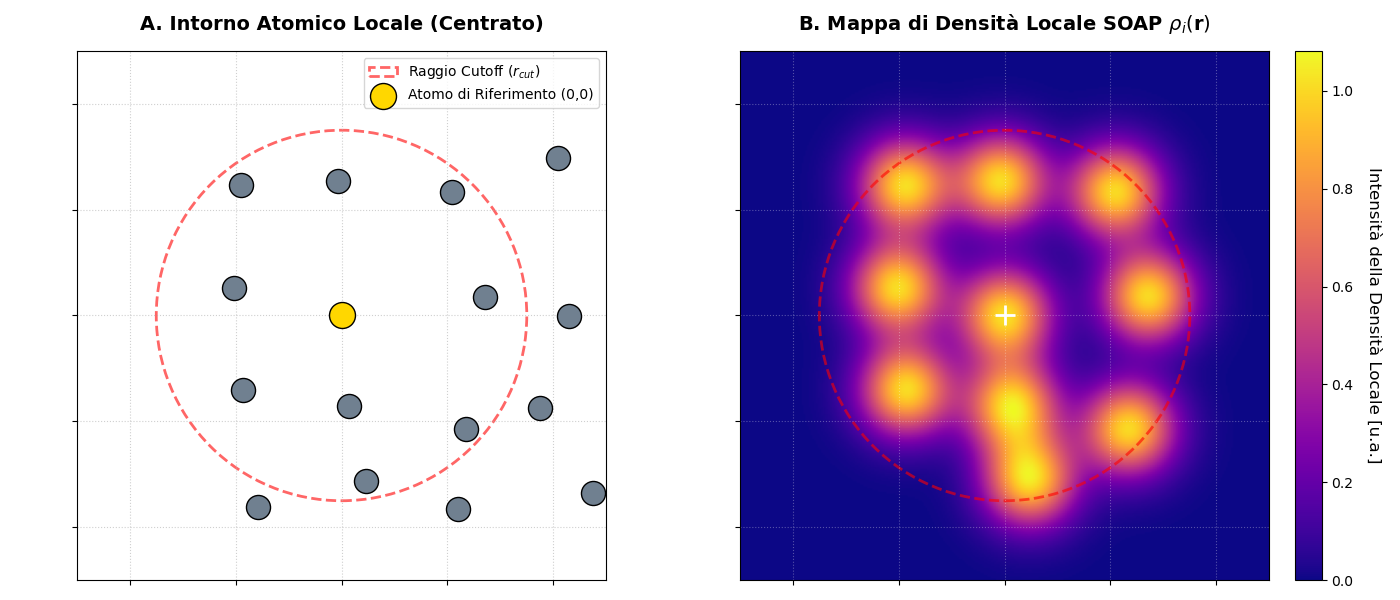
\includegraphics[scale=0.3]{./img/soap-step1-example.png}
    \caption{Rappresentazione generata tramite matplotlib del primo step della procedura SOAP}
    \label{fig:soap-step1-example}
\end{figure}

questa immagine è la somma di tutte le singole mappe prodotte per gli atomi interni al $r_{cut}$, dove è stato preso come riferimento l'atomo color oro posto al centro del sistema di coordinate. Il risultato finale si ottiene prendendo come atomo color oro, a turno, ognuno degli atomi presenti. Per semplicità di rappresentazione la struttura atomica è stata generata aggiungendo rumore ad un cristallo periodico, questo non rappresenta nessuna struttura particolare, è solo una semplice griglia sulle cui intersezioni è stato posizionato un generico atomo.

Il controllo che viene dato dal parametro $\sigma$ della gaussiana è rappresentato nella seguente \ref{fig:soap-step1-example-sigma-big_small}:

\begin{figure}[h]
    \centering
    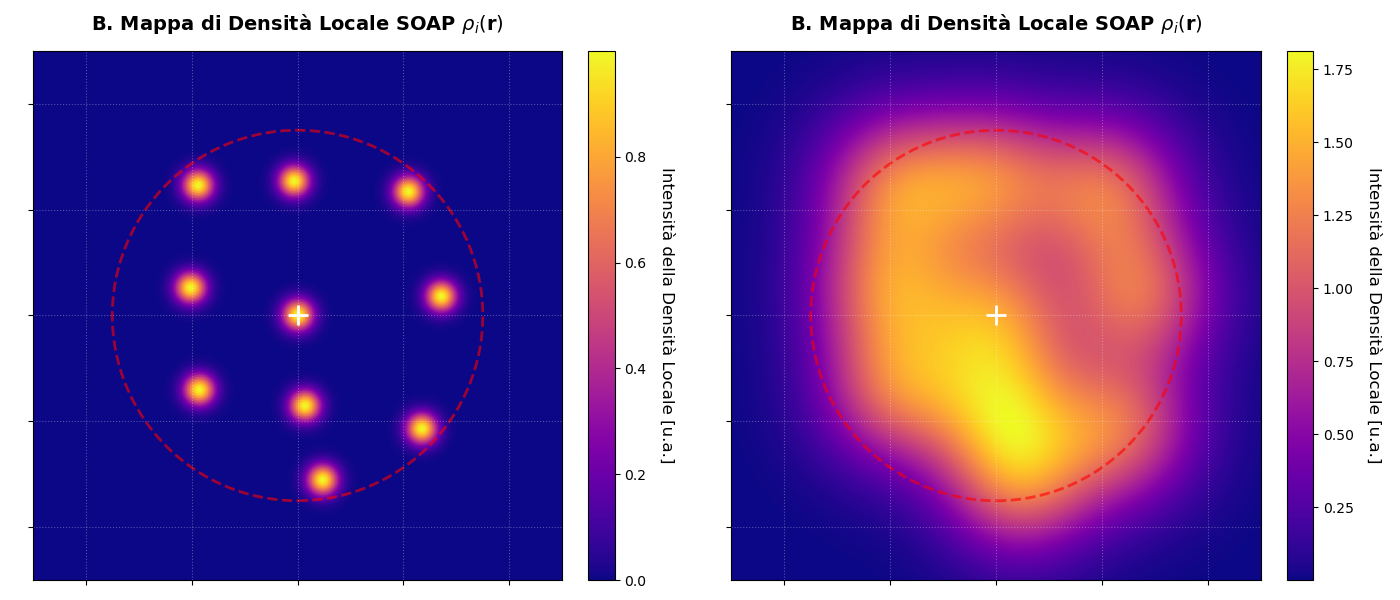
\includegraphics[scale=0.3]{./img/soap-step1-example-sigma-big_small.png}
    \caption{Rappresentazione generata tramite matplotlib del primo step della procedura SOAP per diversi valori del parametro $\sigma$}
    \label{fig:soap-step1-example-sigma-big_small}
\end{figure}

dove il pannello a sx rappresenta il caso di una $\sigma$ eccessivamente piccola e quello a dx il caso di una $\sigma$ eccessivamente grande. In entrambi i casi è possibile notare come l'informazione che se ne ricava non sia adeguata agli scopi descritti sopra. Infatti come detto vogliamo che l'aggiunta di una piccola quantità di rumore non modifichi in modo sensibile il fattore si somiglianza tra le due strutture. Nel primo caso la minima variazione di posizione porta a decretare che gli ambienti sono sensibilmente diversi, mentre nel secondo caso, anche una decisa modifica delle posizioni, porta alla conclusione che i due ambienti siano simili.

Per quanto riguarda il valore di $r_{cut}$, esso controlla il significato che diamo ad "atomi vicini". Se fosse troppo piccolo si perdono informazioni riguardanti la struttura in esame, mentre se troppo grande arriviamo ad avere un vettore di feature complesso e pesante che non fornisce particolari vantaggi.

\subsubsection{Espansione in funzioni di base}
A questo punto ci poniamo di trovare un metodo che ci permetta di riassumere in modo compatto una funzione continua come quella rappresentata dalla mappa di densità. Per fare questo ci procuriamo delle funzioni di base, nel nostro caso radiali e angolari.

L'espansione in serie per la mappa di densità è data da:

\begin{equation}
    \rho_Z(\vec{r}) = \sum_{n=1}^{n_{max}} \sum_{l=1}^{l_{max}} \sum_{m=-l}^{l} c_Z(n,l,m) g(r \,;n) Y(\theta, \phi \,; l,m)
\end{equation}

dove il ; è posto a separatore tra le variabili e i parametri da cui dipendono le funzioni. Il coefficiente $c_Z$ è per la relativa specie in considerazione, come indicato sopra in presenza di specie diverse si costruiscono mappe separate.

In particolare si ha che:

\begin{equation}
    c_Z(; n,l,m) = \int_{\mathbb{R}^3} \mathrm{d}r\, \mathrm{d}\theta\, \mathrm{d}\phi \;\; g(r \,;n) Y(\theta, \phi \,; l,m) \rho_Z(\vec{r}) 
\end{equation}

dove le $g(r \,;n)$ sono funzioni radiali e $Y(\theta, \phi \,; l,m)$ sono armoniche sferiche. Quello che stiamo andando a determinare tramite il coefficiente $c_Z$ è la "misura" della nostra mappa di densità lungo una determinata componente di base, in questo caso funzioni radiali e armoniche sferiche (si utilizzano queste funzioni per le loro proprietà matematiche). Possiamo quindi adesso utilizzare questi coefficienti (un semplice vettore numerico) per ricostruire un oggetto tridimensionale come lo è la mappa di densità. 

In questa sezione non ci dilunghiamo sui dettagli della forma di queste funzioni.

Lo scopo di questo step è quello di semplificare la rappresentazione, come detto passiamo da una struttura tridimensionale complessa ad un singolo vettore numerico. Non abbiamo ancora aggiustato le restanti invarianze, in quanto alla fine di questo step manca ancora l'invarianza per rotazione, la sua risoluzione sarà il cardine dello step successivo.

\subsubsection{Calcolo del power spectrum}

Per rendere la nostra rappresentazione invariante per rotazioni andiamo a calcolare il power spectrum parziale, ottenuto dalla seguente equazione:

\begin{equation}
    p_{Z_1Z_2}(n,n',l) = \pi \sqrt{\frac{8}{2l+1}} \sum_{m=-l}^{l} \overline{c_{Z_1}}(n,l,m) c_{Z_2}(n',l,m)
    \label{eq:power-spectrum}
\end{equation}

dove il primo coefficiente è sotto complessa coniugazione, nel caso si usino solo armoniche sferiche reali, essa diventa superflua. La presenza di $Z_1$ e $Z_2$ indica che questo viene calcolato per ogni coppia unica (indipendentemente dall'ordine) di specie chimiche presenti. Nel contesto del dataset A, quello che si produce è $(Z_{Ta},Z_{Ta})$, $(Z_{O},Z_{O})$ e $(Z_{Ta},Z_{O})$.

Senza entrare nei dettagli, diciamo che questo processo rende il risultato invariante dal punto di vista delle rotazioni, in quanto, le rotazioni possono essere rappresentate tramite matrici unitarie (oppure ortogonali nel caso reale), il processo descritto sopra "trasforma" la matrice di rotazione (con cui possiamo rappresentare la rotazione della mappa di densità rispetto ad un qualunque sistema di riferimento) nella matrice identità, che quindi non modifica il valore del coefficiente.

Le correlazioni che si trovano per valori di $Z_1$ e $Z_2$ diversi tra loro servono per tenere traccia delle posizioni relative delle diverse specie atomiche.

\subsubsection{Risultato finale}

Dopo aver calcolato tutti i vari elementi del power spectrum, si strutturano come un vettore, la cui dimensione viene determinata dalla seguente formula:

\begin{equation}
    \mathrm{dimensione} = (l_{max} + 1) \,\frac{1}{2}\, (S\cdot n_{max}) (S\cdot n_{max} +1)
    \label{eq:formula-dimensione-semplificata}
\end{equation}

Dove $S$ rappresenta il numero totale di specie diverse presenti nel materiale in analisi, $n_{max}$ e $l_{max}$ sono gli stessi parametri precedentemente definiti. 

Per una spiegazione su come ottenere questa formula si veda \autoref{app:dimpowspec}.


\subsubsection{Schema riassuntivo}

Diamo adesso una rappresentazione riassuntiva del processo completo (\ref{fig:schema-riassunto-soap}), compresa anche la possibiltà di dinamica molecolare suddivisa per frames. In particolare, il metodo di archiviazione della struttura di SOAP e la sua indicizzazione / organizzazione è lasciato pienamente in gestione alle librerie utilizzate, notiamo che l'odine del vettore di feature non è trascurabile.

\begin{figure}[h]
    \centering
    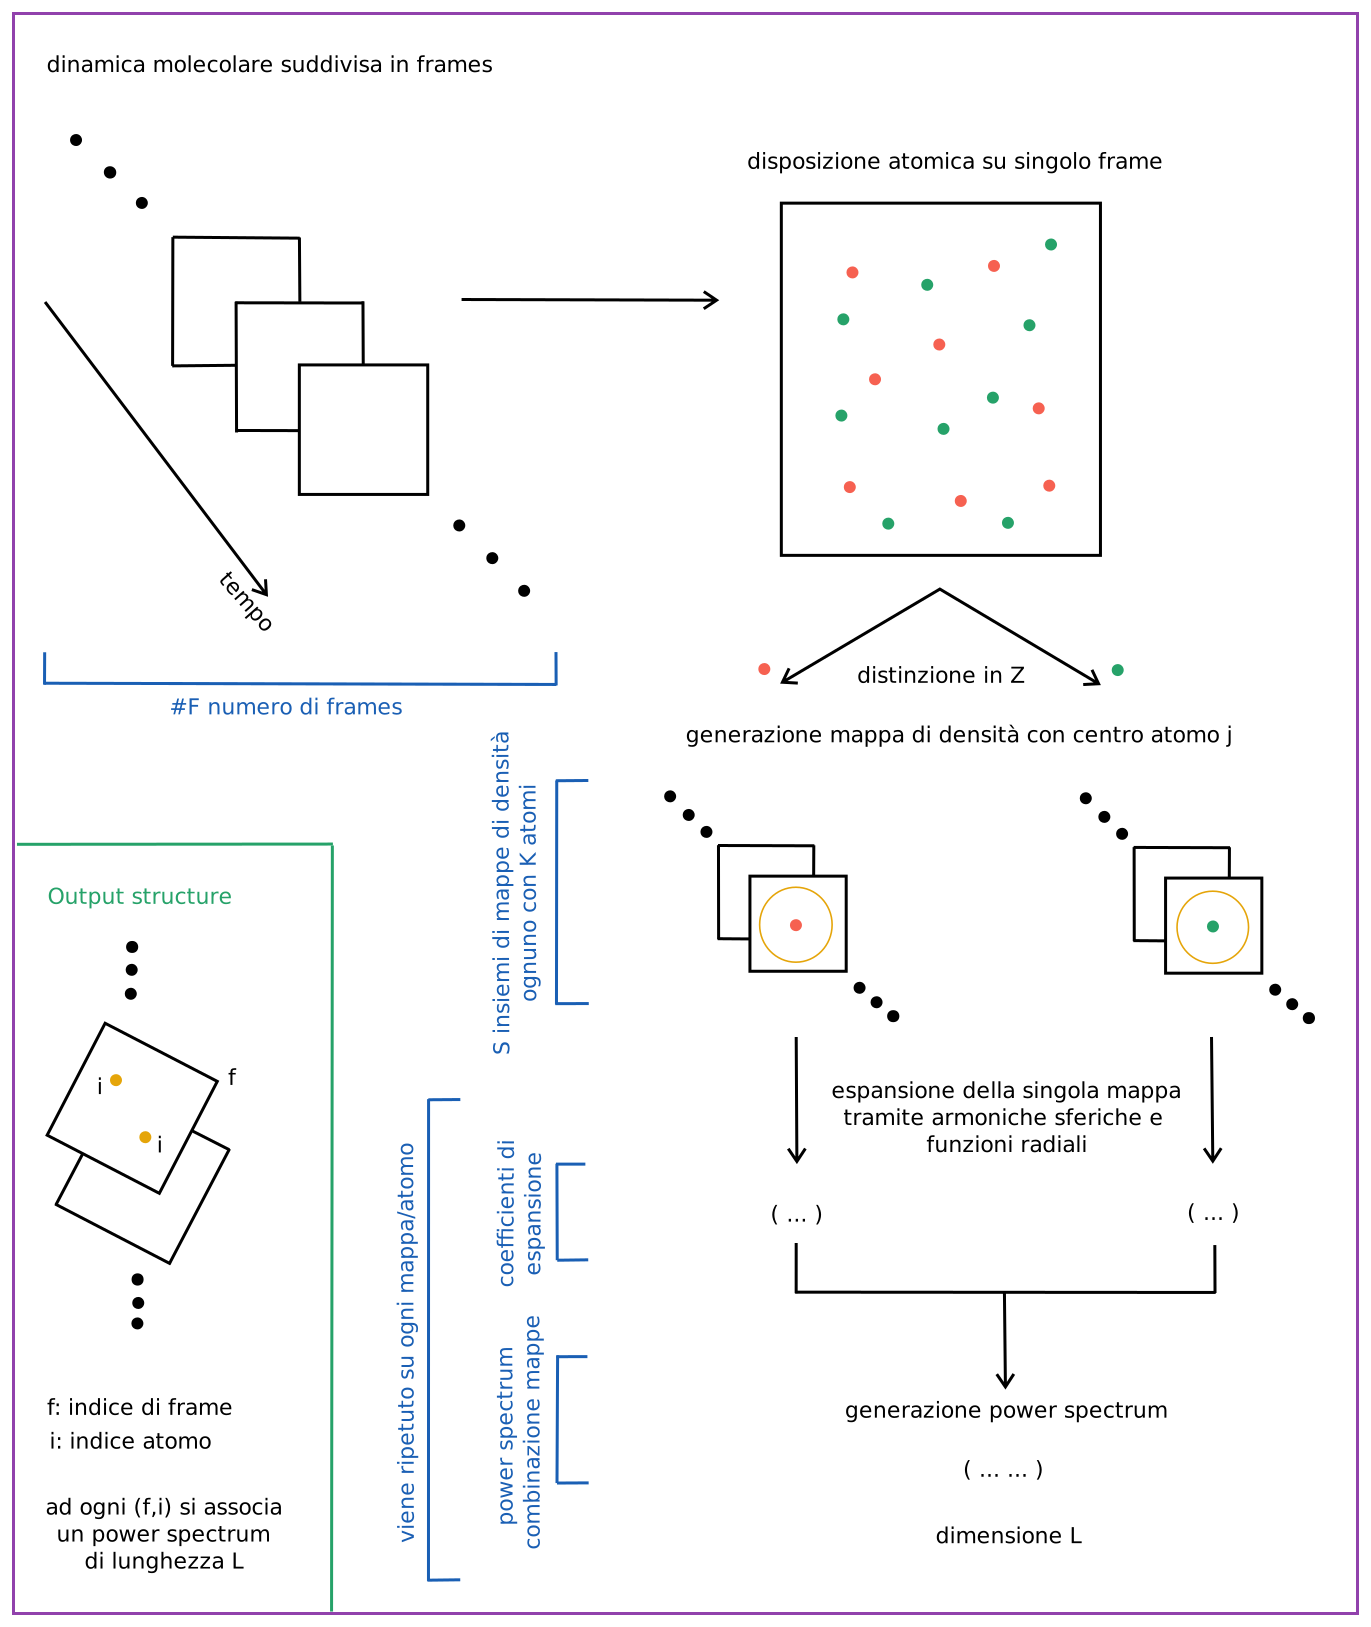
\includegraphics[scale=0.35]{./img/schema-riassunto-soap.png}
    \caption{Rappresentazione schematica della totalità del processo SOAP}
    \label{fig:schema-riassunto-soap}
\end{figure}

\clearpage
